
\chapter{A mnemonic history}

One could argue that the beginning of the SM history coincides with the
beginnings of modern particle physics. Since that depends on unifying
relativity, quantum mechanics, and field theory, one could arguably even take
Maxwell's equations as a starting point. 
There were also many interesting ideas that were not pursued or turned out
not to be correct yet still played some role in the history; I will not
discuss these. In some cases I may miss some discoveries that were also
important but less celebrated.

Given these ambiguities and the fact
that I am not at all a real historian, 
one might call what follows an ``approximate" history.
As I was writing this, I realized that I was trying to tell a story, i.e.
to write it in a way that one development would make sense or feel
motivated given a previous development. Usually that is a bit of an
oversimplification, but it helps me remember why certain discoveries were
significant, where some nomenclature comes from, and what it means. Hopefully it
also helps reveal how physicists think, how we are led to discoveries, and
ultimately why we believe our theories. So with these advantages in mind, I
rather decided to call it a ``mnemonic" history. 

Also while I was writing this, I learned a bunch of facts that I found
interesting but are probably a bit off-topic. Hence this mnemonic history is
densely packed with footnotes. For example I decided to start listing Nobel
prizes for some reason. By the time I realized doing this is tedious and doesn't
teach much, I somehow already felt pot-committed, so I ended up seeing this habit
through to the bitter end. 

\section{The fundamentals}

% pauli, jordan etc 1920s-30s how to quantize fields. 
% Failing to have theory with infinite num of dof,
% then tomonaga, schwinger, dyson, feynman. Can renormalize, QED discovered.
% 1970s golden age: infinites understood through
% renormalization group wilson and kadanoff.

In 1897 J.J. Thomson did experiments with cathode rays\footnote{In a small
vacuum chamber with two electrodes, if a voltage is applied between them,
electrons will move between them. Televisions used to work by cathode ray tubes,
\index{cathode ray tube} where these electrons are deflected by magnetic fields
to make images on the screen.}
from which he concluded that electric charge must be carried by particles
with high charge-to-mass ratio, the electrons\footnote{He received the 1906
Nobel in physics for this work.} 
To explain why atoms are overall electrically neutral, Thomson guessed that
electrons are distributed in a sea of positive charge, which is the
well known {\it plum pudding model}.\index{plum pudding model} This was
disproved by Rutherford in his famous gold foil
experiment~\cite{rutherford_scattering_1911}, in which he discovered
the atomic nucleus. Shortly thereafter, he discovered the
proton~\cite{rutherford_collision_1919}.
Bohr proposed his model~\cite{bohr_constitution_1913}
of hydrogen, supposing it to be made of a proton and an electron, which agreed
well with experiment\footnote{He got the 1922 Nobel for his
contributions understanding atomic structure.}. Extending this theory to 
heavier elements by supposing
they are also made of only protons and neutrons however fails, since e.g. helium
is four times as heavy as hydrogen. This difficulty would not be sorted out
until the early 1930s, when Chadwick discovered~\cite{chadwick_possible_1932}
the neutron\footnote{1935 Nobel for him.}.


These early discoveries successfully explained many details of the atom; however
the fact that atomic nuclei are made of particles with only positive or zero
electric charge still required explanation.
Hence for some time, physicists
knew there must be some {\it strong force}\index{force!strong} that opposes
Coulomb repulsion and binds nucleons into nuclei.
Such particles held together by strong interactions are called
{\it hadrons}.\index{hadron} Nowadays we also use the terms {\it meson}
\index{meson} and {\it baryon}\index{baryon} to refer to hadrons made of
two quarks and three quarks, respectively\footnote{This naming scheme
comes from particle weights. At the time, known leptons were light, 
baryons were heavy, and mesons were somewhere in the middle. In retrospect it
would have been nicer to name them something like $n$-hadrons, but alas it would
take several decades for us to see that hadrons are made of quarks.}.


Around this time, physicists were also beginning to see the particle nature of
light. In particular, Planck proposed~\cite{Planck:1901tja} 
that light may come in discrete packets of
energy in order to avoid the \index{ultraviolet catastrophe}ultraviolet 
catastrophe\footnote{1918 Nobel.}.
Einstein took this proposal seriously~\cite{Einstein:1905cc}, 
and used it to explain the photoelectric
effect\footnote{1922 Nobel for him.}. 
A careful study~\cite{millikan_direct_1916} of the photoelectric effect by 
Millikan showed that
Einstein's interpretation explained the photoelectric effect well\footnote{He
got the 1923 Nobel in part for this reason.}. Finally
Compton showed\footnote{He shared the 1927 Nobel for this.} 
that light scattered from a particle shifts by the Compton
wavelength\index{wavelength!Compton}
\begin{equation}
  \lambda_c=\frac{\hbar}{2mc},
\end{equation}
where $m$ is the target particle's mass, which one can derive by assuming light
is made of particles with zero rest mass~\cite{Compton:1923zz}.
Altogether these discoveries convinced physicists light behaves as a particle
at short enough length scales, which is the usual photon.\index{photon}


If light is to be quantized, it requires a theory that knows about both quantum
mechanics and special relativity, i.e. it needs QFT. 
The standard line of thinking can be cast in this way: One starts with
the Schr\"odinger 
equation~\cite{Schrodinger:1926gei,Schrodinger:1926vbi,Schrodinger:1926qnk,Schrodinger:1926xyk}
for a spinless, non-relativistic particle
of mass $m$ in the position basis,
\index{Schr\"odinger equation}
\begin{equation}
i\hbar\partial_t\psi=-\frac{\hbar^2}{2m}\nabla^2\psi.
\end{equation}
If we instead use a relativistic Hamiltonian and square the differential
operators on each side, we get the 
{\it Klein-Gordon equation}~\cite{Klein:1926tv,gordon_comptoneffekt_1926}
\index{Klein-Gordon equation}
\begin{equation}
-\hbar^2\partial_t^2\psi=\left(-\hbar^2c^2\nabla^2+m^2c^4\right)\psi.
\end{equation} 
While this is at least relativistically sensible, one can show that this
squaring of operators
leads to state normalization being time-dependent, i.e. probability is not
conserved. The situation was finally rescued by Dirac\footnote{Dirac
and Schr\"odinger shared the 1933 Nobel.}, who realized that
one could have a relativistically sensible equation that is first-order
in its operators by introducing some matrices and a spin component
to the wavefunction~\cite{Dirac:1928hu,Dirac:1928ej}. The result is the 
{\it Dirac equation}\index{Dirac equation}
\begin{equation}
i\hbar\slashed{\partial}\psi=mc\psi.
\end{equation}

The corresponding Hamiltonian for the Dirac equation is traceless, which
tells you that the energy eigenvalues cancel out, i.e. 
it suggests there are states of
negative energy. These negative energy states indicate that the theory
has no ground state. In order to prevent this infinite cascade into increasingly
negative energies, he speculated that these infinitely many states are already
occupied, which is referred to as \index{Dirac sea}the {\it Dirac sea}; 
the Pauli exclusion principle then prevents this infinite descent. 
If an electron in the sea were excited, it would leave behind a vacancy
that would manifest itself as a positively charged particle. This was the
prediction of the existence of the \index{positron}positron, which
was discovered\footnote{1936 Nobel.} in 1932 by Anderson~\cite{Anderson:1933mb}.
Later St\"uckelberg~\cite{Stueckelberg:1941rg} and
Feynman~\cite{feynman_theory_1949} would introduce the modern interpretation
of the positron: rather than being a hole left in the Dirac sea,
the previously negative energy states are to be understood as the
positive energy states of a different particle.


One of the last kinds of fermions needed to complete our particle collection
are the neutrinos. Before 1930, there was a problem with $\beta$-decay
\index{decay!beta} 
which is any decay emitting an $e^+$ or $e^-$ from
an atomic nucleus: Energy was not conserved. In particular if one assumes
a general $\beta$-decay process functions like
\begin{equation}
  A\to B+e^-,
\end{equation}
one can use conservation of four-momentum to find the electron energy.
The measured energy was found to fluctuate and be smaller than what four-momentum
conservation delivers. Pauli
suggested\footnote{Rather than being documented in a publication, this seems to
come from a letter written by Pauli addressed to a conference in T\"ubingen.
It opens, ``Liebe Radioaktive Damen und Herren".} that this missing energy
lies with an as-yet-undetected, weakly interacting particle, the
electron neutrino. The electron neutrino would not be 
discovered\footnote{1995 Nobel.}\index{neutrino!electron}
until the mid 1950s by Cowan and Reines~\cite{Cowan:1956rrn}.

\section{Weak and strong forces}

\index{interaction!weak}
In the early 1930s, Fermi published\footnote{Apparently he originally attempted
to publish it in {\it Nature}, but they rejected it because
it because ``it contained speculations too remote from reality to be of interest
to the reader".} his theory of the 
\index{decay!beta}$\beta$-decay~\cite{fermi_tentativo_1934}
\begin{equation}
  n\to\text{p}+e^-+\bar{\nu}_e.
\end{equation}
He introduced an effective 4-point interaction directly linking the four
particles in the above process.
Shortly thereafter, Yukawa~\cite{yukawa_interaction_1935} put forward that this
interaction should include another field with corresponding quantum that
mediates this interaction\footnote{Nowadays we designate as
{\it Yukawa interaction} any interaction between
Dirac fields and scalar fields of the form\index{interaction!Yukawa}
$g\bar{\psi}\phi\psi$ or $g\bar{\psi}i\gamma_5\phi\psi$.}, 
sort of like how the photon mediates the
electromagnetic interaction. Another salient point of this paper is
the introduction of the {\it Yukawa potential}\index{potential!Yukawa}
giving the potential of a gauge boson of mass $m$:
\begin{equation}
  V(r)=-g^2\frac{e^{-\alpha m r}}{r}.
\end{equation}
Here $g$ is the gauge coupling and $r$ is the interaction range. One sees that
massless gauge bosons have a Coulomb-like potential, while massive ones
are suppressed exponentially\footnote{One can also show that the Fourier
transform of this potential is the propagator, which we will discuss later.},
which gives an explanation why the weak force has a short interaction range. 
Besides already hinting massive weak bosons, this paper is considered to be
one of the first theories of the strong force; from this perspective the
proton and neutron exchange massive mesons, which therefore have a limited
interaction range\footnote{1949 Nobel.}.

\begin{figure}
  \centering
  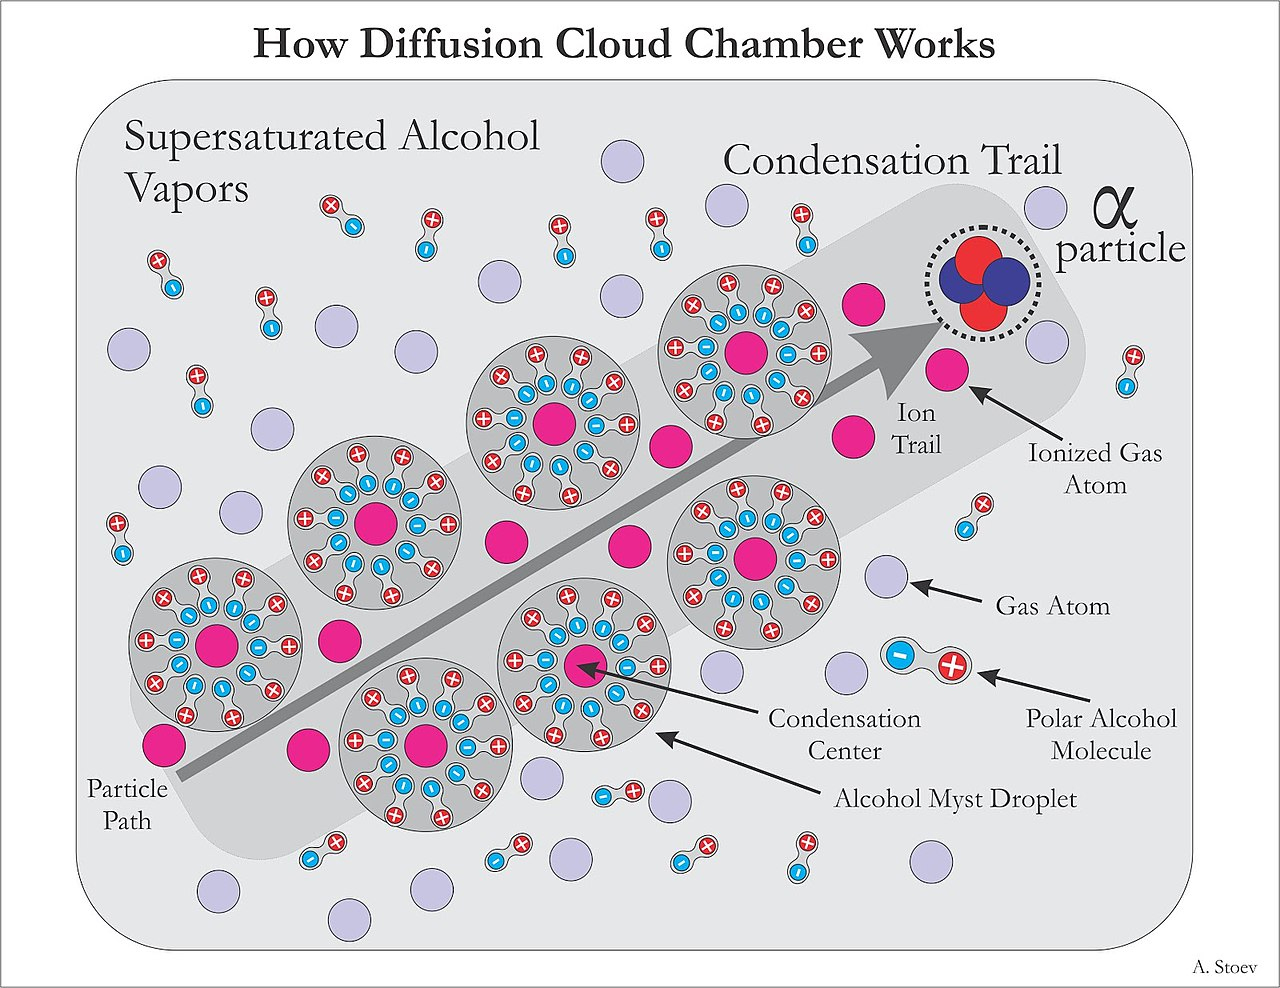
\includegraphics[width=\linewidth]{figs/Diffusion_Cloud_chamber_explained.jpg}
  \caption{Cloud chambers consist of a sealed environment with some vapor
           of e.g. alcohol. As a charged particle moves through the vapor, it knocks
           electrons off the gas; the resulting ions attract the polar molecules,
           which leaves a visible trail for a short time. To identify particles,
           you can see e.g. if they were deflected. C. T. R. Wilson is generally 
           credited as the inventor of cloud chambers, and he shared the 1927 Nobel
           in physics for it. They were extremely popular to use in experiment
           for finding particles until the later invention of the bubble chamber.
           Image taken from Wikipedia~\cite{wiki_cloud}.}
  \label{fig:cloud}
\end{figure}

An early experimental search of cosmic ray\footnote{A {\it cosmic ray} is a high
energy proton or atomic nucleus that originates somewhere from space. They were
discovered in the early 1910s by Hess, which got him the 1936 Nobel.}
\index{cosmic ray} measurements using
cloud\index{cloud chamber} chambers (see \figref{fig:cloud}) 
found the muon~\cite{neddermeyer_note_1937}, which was originally 
mistaken\footnote{Indeed the muon and pion masses are pretty close to each
other, sitting at about 106~MeV and 140~MeV, respectively.}
as the meson that Yukawa suggested. An experiment in the late 1940s showed that
the muon does not interact very strongly with atomic
nuclei~\cite{conversi_disintegration_1947}, which rules it out as the strong
force mediator. Thankfully for Yukawa the pion was
discovered~\cite{lattes_processes_1947} in 1947\footnote{And got Powell
the 1950 Nobel for it. It is actually a bit puzzling that he is the only
recipient of this prize, most obviously because only three other scientists were
on his team. Furthermore this prize credits him for his ``development of
photographic method for studying nuclear processes", even though this method was
pioneered by other physicists such as Blau and Wambacher.}.


\index{interaction!strong}
In the late 1940s and early 1950s, the {\it kaon} ($K$)~\cite{rochester_evidence_1947}
\index{meson!K} and {\it lambda} ($\Lambda$)~\cite{hopper_evidence_1950}
\index{baryon!lambda} hadrons were discovered. A kaon
consists of light quark and a strange, while a lambda baryon binds two light
quarks with one from a higher generation. {\it Strangeness}\footnote{We now 
\index{strangeness}
identify strangeness $S$ as
$$
  S\equiv\#\,\text{anti-strange quarks}-\#\,\text{strange quarks}.
$$}
was originally proposed as a conserved quantity to explain the relatively long
lifetimes of these particles~\cite{pais_remarks_1952,gell-mann_isotopic_1953,
pais_baryon-meson-photon_1953,tadao_charge_1953}.
Ne'eman~\cite{neeman_derivation_1961},
Gell-Mann~\cite{gell-mann_symmetries_1962}, and
Zweig~\cite{zweig_su3_1964} proposed\footnote{Gell-Mann would receive the 1969
Nobel for his contributions to understanding elementary particle
classification.} that these hadrons could be classified
according to the irreducible representations of $\SU(3)$, a viewpoint which
Gell-Mann called the \index{eightfold way}{\it eightfold way}\footnote{This
name is inspired by the eightfold path of Buddhism.}, examples of which are
illustrated graphically in \figref{fig:eightfold}. Gell-Mann
referred to the fundamental units as {\it quarks}\footnote{Gell-Mann borrows
this name from an excerpt of James Joyce's {\it Finnegan's Wake} that begins
``Three quarks for Muster Mark".
Gell-Mann was a bit of a fanciful guy I guess.}.
At first it was not clear that this quark viewpoint was more than a
purely mathematical construction, however deep inelastic
scattering\index{scattering!deep inelastic}
experiments at the Stanford Linear Accelerator (SLAC) showed that
protons are made of smaller particles, and are therefore not
elementary~\cite{bloom_high-energy_1969,breidenbach_observed_1969}.
This alone did not convince the community that quarks were 
real\footnote{For a while it was fashionable to refer to rather refer to
nucleon constituents as {\it partons}\index{parton}, a term coined
by Feynman.}, but
subsequent discoveries would solidify the quark model.

\begin{figure}[t]
  \centering
  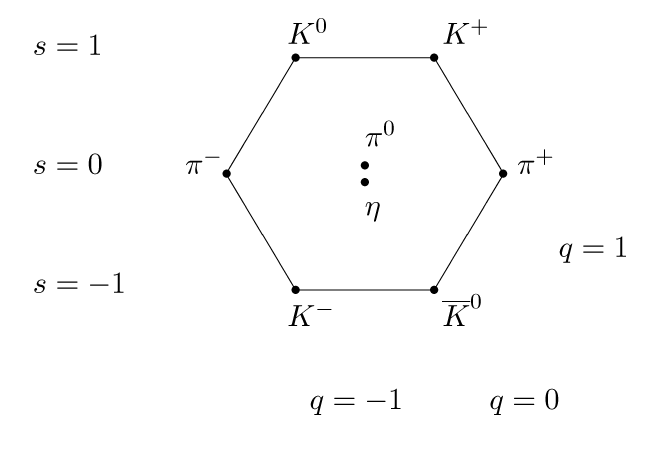
\includegraphics[width=0.48\linewidth]{figs/Meson_octet.png}
  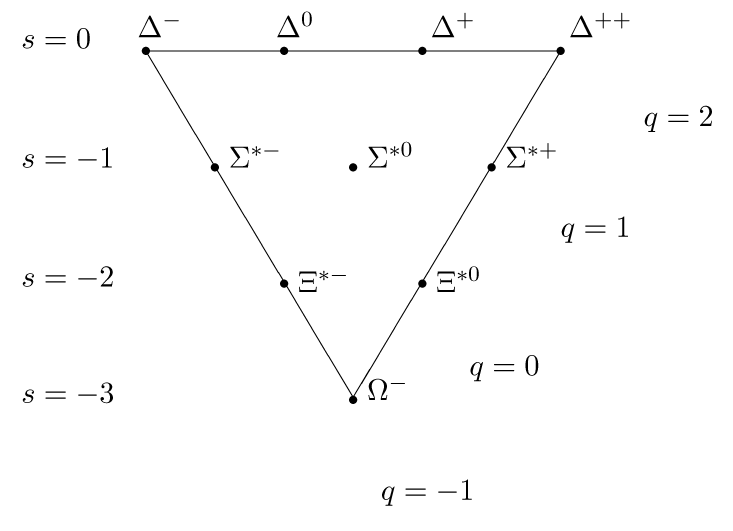
\includegraphics[width=0.48\linewidth]{figs/Baryon_decuplet.png}
  \caption{{\it Left}: Spin-0 pseudo-scalar meson octet. {\it Right}:
           Spin-3/2 baryon decuplet. The $s$ represents strangeness,
           with all particles in the same horizontal row having the
           same strangeness. Electric charge is represented by $q$,
           with all particles along the diagonal having the same
           electric charge. Images taken from
           Wikipedia~\cite{wiki_eightfold}.}
  \label{fig:eightfold}
\end{figure}

From here it was shown possible to formulate a QFT for the strong interaction
based on $\SU(3)$~\cite{fritzsch_advantages_1973}, which we
call quantum chromodynamics (QCD).\index{quantum chromodynamics}
The mediators are called
{\it gluons}\index{gluon} with the adjoint representation delivering
eight possible color combinations.
Gross, Wilczek~\cite{gross_d.j._ultraviolet_1973} and
Politzer~\cite{politzer_reliable_1973} demonstrated
{\it asymptotic freedom}\footnote{They got the 2004 Nobel for this.}
\index{asymptotic freedom} in this QFT, i.e. they showed that the
strong coupling decreases with increasing interaction strength, which is
consistent with the fact that one does not observe free quarks\footnote{At
least not at typical temperatures and densities.}.
This theoretical observation is buttressed by strong coupling
expansions in the lattice formulation, introduced by 
Wilson~\cite{wilson_confinement_1974}, which show that the potential
energy between two infinitely heavy quarks grows linearly with
increasing separation.
%creutz_monte_1980
%wilson_RG 1 and 2

We round out this section with a short timeline of discoveries of the
remaining QCD particles. In 1974 the discovery of the
$J/\Psi$-meson\index{psion} or {\it psion}\footnote{The $J/\Psi$ consists
of a $\bar{c}c$ pair. This is also sometimes called {\it charmonium}.
\index{charmonium}} at both Brookhaven National Lab (BNL) and
SLAC~\cite{augustin_discovery_1974,aubert_experimental_1974} demonstrated
the existence of the charm quark\footnote{Richter and Ting got the 1974
Nobel prize in physics for this.}, adding further evidence to
the validity of the quark model. The $J/\Psi$ discovery marks the beginning of a
period of rapid discoveries in particle physics sometimes referred to as the
``November Revolution".\index{November Revolution} The existence of the bottom
quark was demonstrated in 1977 at Fermilab~\cite{herb_observation_1977} when the
$Y$-meson\footnote{A $Y$-meson\index{meson!Y} is a $\bar{b}b$ bound state. This is
sometimes called \index{bottomonium}{\it bottomonium}.} was discovered.
In 1979 we found experimental evidence for the
gluon via indirect observations~\cite{barber_discovery_1979} at the
Deutsches Elektronen-Synchrotron (DESY). In part because it is the
heaviest quark, the top quark would not be discovered until
1995~\cite{abachi_observation_1995,abe_observation_1995}
at Fermilab.


\section{Unification}


In the mid 1950s, Lee and Yang~\cite{lee_question_1956} suggested possible
experimental tests to search for parity violation in weak interaction 
processes\footnote{Lee and Yang won the 1957 Nobel prize for this.}.
Shortly thereafter, Wu et al.~\cite{wu_experimental_1957} demonstrated parity
violation in the $\beta$-decay of \ce{^{60}Co},
a result which was verified by Garwin et al.~\cite{garwin_observations_1957}. 
The theory of the weak interaction was extended by Gell-Mann and
Feynman~\cite{feynman_theory_1958} to accommodate parity violation by
introducing vector-axial currents.
That $\beta$-decay proceeds through vector-axial currents was
experimentally verified shortly thereafter~\cite{goldhaber_helicity_1958}.


The unification of the weak and electromagnetic forces began already with
Glashow in 1961~\cite{glashow_partial-symmetries_1961}, where
he puts forward the $\SU(2)\times \U(1)$ symmetry group. 
Still, this theory was not known to be renormalizable.
Also the weak interaction is short range, but this suggests that the mediating boson 
should be massive according to Yukawa. On the other hand, 
massive gauge bosons superficially spoil gauge invariance.


In superconductivity, Ginzburg-Landau theory~\cite{ginzburg_theory_1950}
gives solutions with effective mass. Nambu applied\footnote{2008 Nobel prize.} 
this to particle
physics~\cite{nambu_axial_1960,nambu_dynamical_1961,nambu_dynamical_1961-1},
but this implied the existence of Goldstone modes that are not observed.
Higgs~\cite{higgs_broken_1964} and Brout and Englert~\cite{englert_broken_1964}
noticed\footnote{Higgs and Englert received the 2013 Nobel for this.} 
that by strategically choosing 
the gauge, one can simultaneously
eliminate the Goldstone modes, add a mass term to gauge bosons, and a scalar
boson, the Higgs boson.\index{boson!Higgs}


The original Higgs-Brout-Englert mechanism was demonstrated only for massive
QED; Kibble extended this idea to non-abelian
groups~\cite{kibble_symmetry_1967}. Weinberg~\cite{weinberg_model_1967}
and Salam~\cite{salam_weak_1968} applied Kibble's results to Glashow's
$\SU(2)\times\U(1)$ idea\footnote{And shared the 1979 Nobel for it.}. 
They demonstrated that one can generate masses
for weak gauge bosons along with electrons and muons, while still leaving
neutrinos massless. This approach also predicted neutral weak currents,
which were discovered shortly thereafter by the Gargamelle
experiment~\cite{hasert_observation_1974}. The $W$ and $Z$ bosons would
be discovered at the European Organization for Nuclear Research (CERN)
in the early 1980s~\cite{aubert_ratio_1983,arnison_experimental_1983}.


In 1963, Cabibbo introduced the {\it Cabibbo angle}\index{Cabibbo angle} allowing
for quark mixing in weak interactions~\cite{cabibbo_unitary_1963} to
explain the lifetimes of heavier hadrons. The suppression of flavor changing
neutral currents was explained in the early 1970s through the GIM\index{GIM mechanism}
mechanism~\cite{glashow_weak_1970}, but in order for this mechanism to work,
one needed full doublets of quarks and leptons.
Then Kobayashi and Maskawa predicted the existence of a third
generation~\cite{kobayashi_cp_1973}, since three quark generations are the
minimal amount needed to allow CP violation in the quark sector\footnote{They
shared the 2008 Nobel along with Nambu.}. The full quark mixing matrix
is known as the CKM matrix.\index{CKM matrix} Neutrino mixing is also handled
through a mixing matrix, the so-called PMNS matrix.\index{PMNS matrix} 


In the early 1970s, t'Hooft and Veltman
showed\footnote{1999 Nobel prize for them.} these theories are
renormalizable~\cite{t_hooft_regularization_1972}. Together the Higgs mechanism
and renormalizability of the SM allow one to consistently generate gauge boson
masses while ensuring its applicability at all energy scales.
Furthermore CERN's 2012 discovery of the Higgs 
boson~\cite{aad_observation_2012,chatrchyan_observation_2012} shows that Higgs mechanism
corresponds to reality, rather than being just a mathematical trick to 
consistently approach massive elementary particles.


\bibliographystyle{unsrtnat}
\bibliography{bibliography}
